% !TEX root = ./main.tex
% !TEX encoding = UTF-8 Unicode
% !TEX program = pdflatex
% !TeX spellcheck = it_IT

\chapter{Influence Maximization}
In questo capitolo verrà mostrata la creazione del grafo relativo alla \textit{Social Network}
e l'algoritmo di \textit{Influence Maximization} applicato su di esso.

\section{Creazione del grafo}
Nel precedente capitolo è stata illustrata la caratterizzazione dei nodi (lo score
assegnato ad ogni utente) e la creazione delle relazioni tra essi, con il relativo
peso associato.\\
Per la creazione del grafo è stato utilizzato il framework \textit{\textbf{Graphx}},
il quale permette di definire un oggetto di tipo grafo a partire da un \textit{VertexRDD},
contenente i nodi, e un \textit{EdgeRDD} contenente le relazioni con i relativi pesi.\\
Di seguito è riportato il codice.

\begin{figure}[!htbp]
	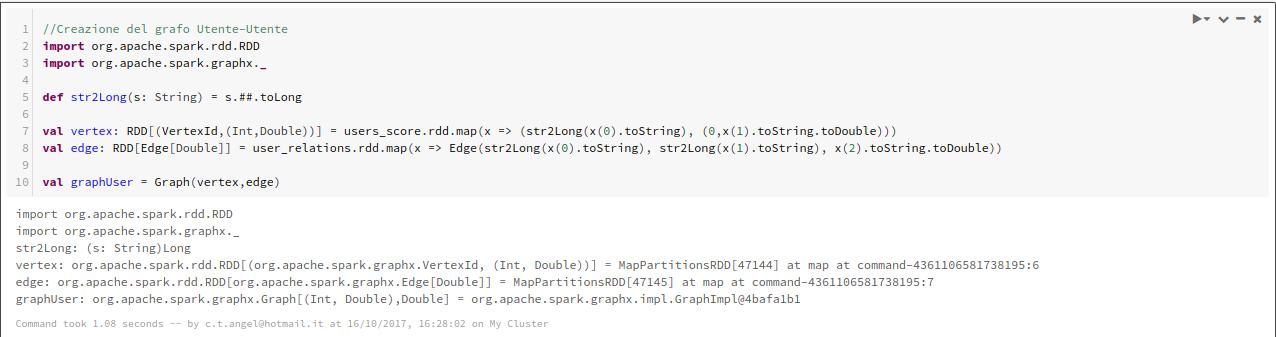
\includegraphics[width=1\linewidth,keepaspectratio]{command_17}
	\caption{Creazione del grafo}
	\label{command_17}
\end{figure}
\clearpage

\section{Algoritmo di Influence Maximization}
L'idea di base dell'algoritmo di Influence Maximization è la seguente: dato il
grafo delle rete sociale ottenuto, avente uno score per ogni nodo ed un peso per
ogni arco, individuare un numero finito di nodi da cui iniziare la copertura del
grafo e propagare l'influence, se e solo se, tale valore supera una soglia prefissata.\\
Per mostrare l'algoritmo utilizzato si consideri il grafo d'esempio in figura.

\begin{figure}[!htbp]
  \begin{center}
    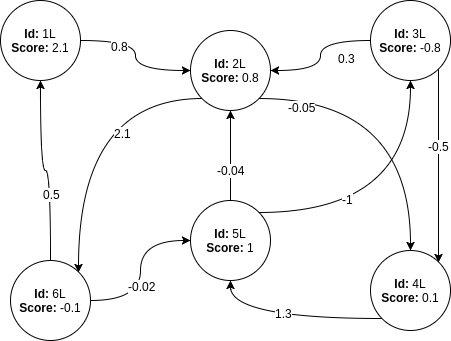
\includegraphics[width=0.6\linewidth,keepaspectratio]{step0}
  	\caption{Grafo d'esempio}
  	\label{step0}
  \end{center}
\end{figure}

\clearpage

Adesso, a fini illustrativi, si considera come nodo di partenza quello avente
score maggiore(evidenziato in verde).\\
Successivamente, invece, verrà illustrata la tecnica utilizzata nell'algortimo di \textit{spread}
per selezionare i nodi di partenza.\\
Nelle figure a seguire, tutti i nodi influenzati saranno evidenziati in verde.
\begin{figure}[!htbp]
  \begin{center}
    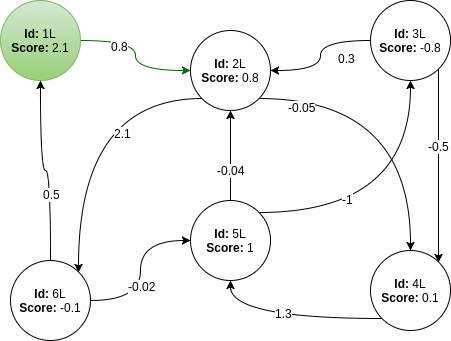
\includegraphics[width=0.6\linewidth,keepaspectratio]{step1}
  	\caption{Scelta nodo di partenza}
  	\label{step1}
  \end{center}
\end{figure}
\clearpage
Ciò che adesso viene illustrato è il meccanismo di diffusione dell'influenza nel
grafo.\\
Il nodo di partenza ha un solo arco in uscita, quindi invierà un messaggio contenente il proprio valore e
la media tra il proprio score ed il peso associato all'arco.\\
Il messaggio ha la seguente struttura $(score\_src, 0.5*score\_src+0.5*weight\_edge)$.\\
Una volta ricevuto il messaggio, il nodo destinazione controlla se il secondo valore è maggiore di una certa soglia,
ad esempio 0.\\
Qualora il confronto risulti positivo, il nodo viene marcato come influenzato ed il
suo score sarà aggiornato con il minimo tra lo score sorgente(moltiplicato per un costante 0.5) ed il proprio score.\\
In \figurename~\ref{step2} è riportato il primo step.\\In particolare si noti che il nodo
risulta essere influenzato, ma il suo score non varia essendo il minimo tra 2.1*0.5 e 0.8.

\begin{figure}[!htbp]
  \begin{center}
    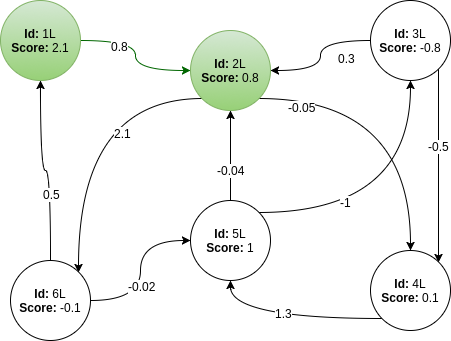
\includegraphics[width=0.6\linewidth,keepaspectratio]{step2}
  	\caption{Passo uno}
  	\label{step2}
  \end{center}
\end{figure}
\clearpage
L'algoritmo continua fintantoché tutti i nodi sono influenzati oppure non esistono più cammini percorribili.\\
Quindi tornando all'esempio, nel secondo step saranno influenzati i nodi \textbf{6L} e \textbf{4L}.

\begin{figure}[!htbp]
  \begin{center}
    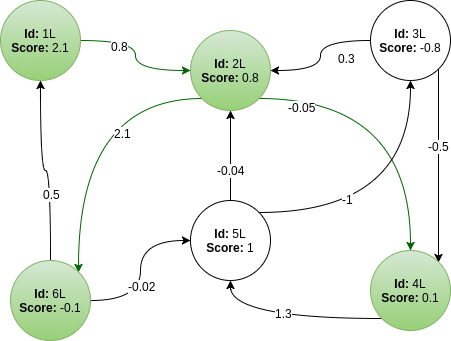
\includegraphics[width=0.6\linewidth,keepaspectratio]{step3}
  	\caption{Passo due}
  	\label{step3}
  \end{center}
\end{figure}
\clearpage
Nel terzo step, si noti che il nodo \textbf{5L} ha due archi in ingesso, sui quali riceve simultaneamente
due messaggi.\\
In tal caso è considerato valido il messaggio avente il secondo campo maggiore.\\
Lo score del nodo 5L è aggiornato, essendo maggiore del valore ricevuto nel messaggio.\\
\begin{figure}[!htbp]
  \begin{center}
    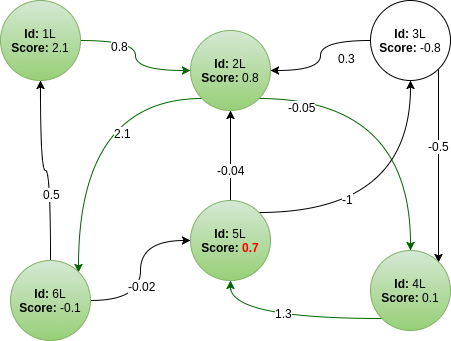
\includegraphics[width=0.6\linewidth,keepaspectratio]{step4}
  	\caption{Passo tre}
  	\label{step4}
  \end{center}
\end{figure}
\clearpage

Nel ultimo step, si noti che il nodo \textbf{3L}, marcato di rosso, non è stato influenzato
in quanto il valore non supera la soglia.
\begin{figure}[!htbp]
  \begin{center}
    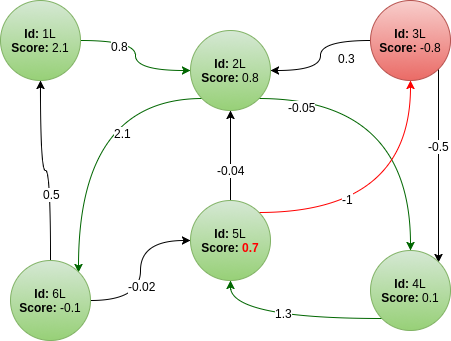
\includegraphics[width=0.6\linewidth,keepaspectratio]{step5}
  	\caption{Passo quattro}
  	\label{step5}
  \end{center}
\end{figure}
\clearpage
\subsection{Scelta degli utenti di partenza}
In questo paragrafo sarà discusso il criterio con cui sono stati scelti gli utenti
di partenza per l'algoritmo di Influence Maximization.\\
In teoria andrebbero testate tutte le possibili combinazioni, in maniera esaustiva,
ma ciò richiederebbe un effort computazionale troppo elevato.\\
L'idea di base è quella di considerare solo un subset di combinazioni, non casuale,
in cui ogni combinazione è costruita con nodi sufficientemente distanti
tra loro, così da assicurare il più possibile una copertura omogenea del grafo.\\
Nel caso in esame, essendo una social network, è possibile utilizzare
come metrica di distanza tra i nodi la loro appartenenza a differenti cluster.\\
Utilizzando un'algoritmo di clustering per grafi, è possibile selezionare
i cluster più fitti e successivamente considerare solo gli N nodi con score maggiore.\\
A causa dei limiti hardware imposti da Databricks, è stato scelto di usare un
massimo di 5 cluster e 2 nodi ciascuno, ottenendo così 32 combinazioni differenti.\\
L'algoritmo di clustering scelto è \textbf{Markov Cluster(MCL)}, basato sulle
catene di Markov.\\
\subsubsection*{Markov Cluster(MCL)}
Per individuare un cluster in un grafo, MCL utilizza una \textbf{matrice stocastica}(matrice
avente elementi non negativi e somma sulle righe o sulle colonne unitaria) ed
il concetto di \textbf{random walks}(cammini casuali tra i nodi).\\
I random walks tra due nodi sono più frequenti se essi appartengono allo stesso gruppo.\\
Studiando la probabilità che un nodo raggiunga un altro nodo del grafo, è possibile
associarlo al cluster corretto.\\
L'algoritmo\footnote{Stijn van Dongen. A stochastic uncoupling process for graphs.
Technical Report INS-R0011, National Research Institute for Mathematics and Computer
Science in the Netherlands, Amsterdam, May 2000.} è diviso in tre fasi, le prime
due simulano i random walks mentre la terza effettua una test di convergenza.\\
Nel dettaglio:
\begin{itemize}
  \item \textbf{Expansion}: calcola il quadrato della Matrice Stocastica;
	\item \textbf{Inflation}: applica il prodotto di Hadamard sulla matrice stocastica
	(prodotto tra due matrici, in cui la risultante ha ad ogni valore \textit{ij} il prodotto
	degli elementi \textit{ij} delle matrici originali e la loro stessa dimensione).
\end{itemize}
Le fasi di Expansion e Inflation sono eseguite in loop più volte finchè un criterio
di \textit{Convergenza} stabilisce che la nuova matrice risultante sia stabile
rispetto l'iterazione precedente.\\
Nel caso non si ottenga la convergenza, esiste un criterio di stop di "sicurezza"
per evitare l'esecuzione dell'algoritmo all'infinito(o per un periodo
inaccettabilmente elevato).\\
Di seguito è riportato il codice in cui è utilizzato tale algoritmo.
\begin{figure}[!htbp]
  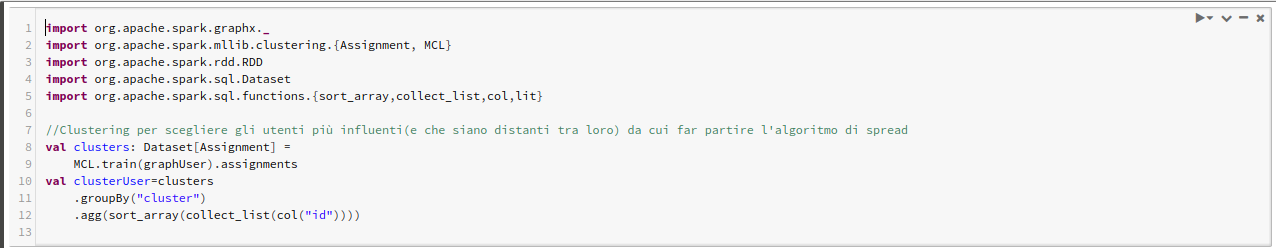
\includegraphics[width=1\linewidth,keepaspectratio]{command_18}
  \caption{Clustering}
  \label{command_18}
\end{figure}

\clearpage
Dato che l'algoritmo di clustering utilizzato non considera i valori presenti nei
nodi, al termine del processo di clustering è necessario recuperarne lo score.\\
Di seguito è riportato il codice per l'estrazione dei nodi di partenza.
\begin{figure}[!htbp]
  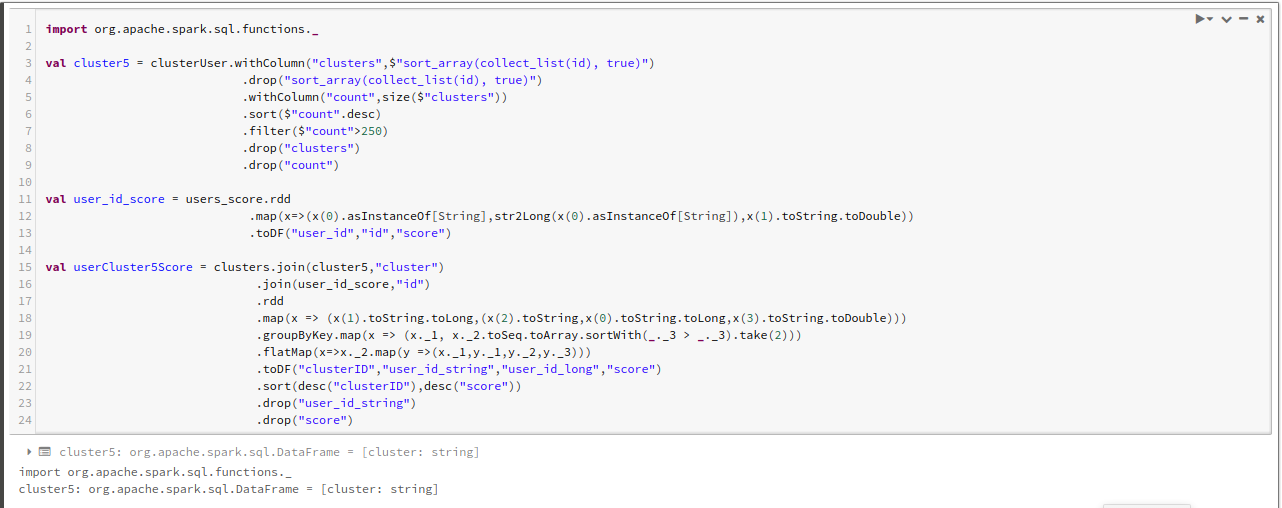
\includegraphics[width=1\linewidth,keepaspectratio]{command_20}
  \caption{Nodi di partenza}
  \label{command_20}
\end{figure}

Nella seguente figura è riportato il codice per la creazione delle combinazioni dei
nodi.
\begin{figure}[!htbp]
  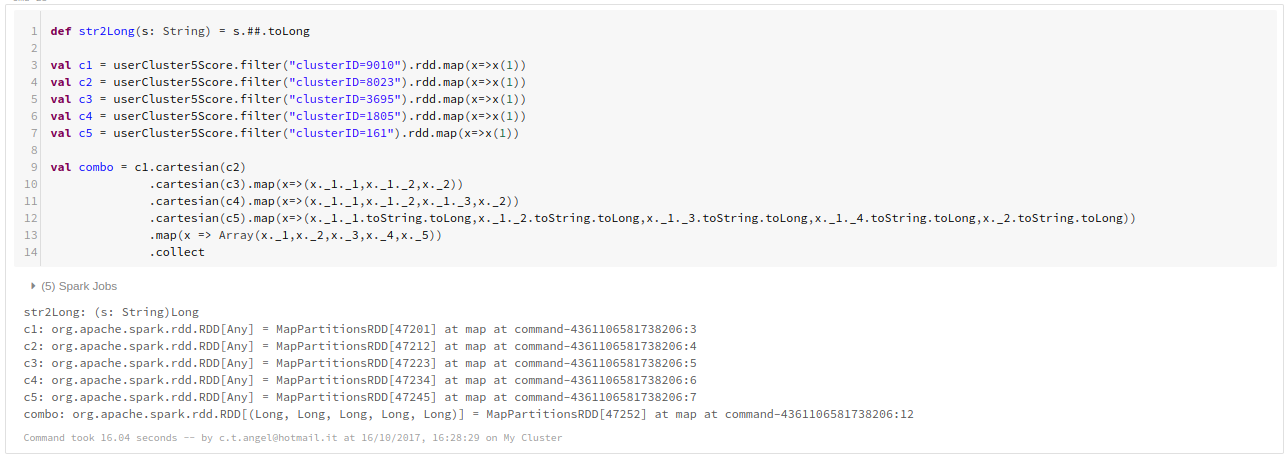
\includegraphics[width=1\linewidth,keepaspectratio]{command_23}
  \caption{Combinazioni dei Nodi}
  \label{command_23}
\end{figure}
\clearpage

\subsection{Scelta della soglia}
La soglia utilizzata per stabilire se un nodo è stato influenzato dal precedente
oppure no, è calcolata come media tra la mediana degli score degli utenti e la
mediana dei pesi degli archi, come mostrato in \figurename~\ref{command_24}

\begin{figure}[!htbp]
  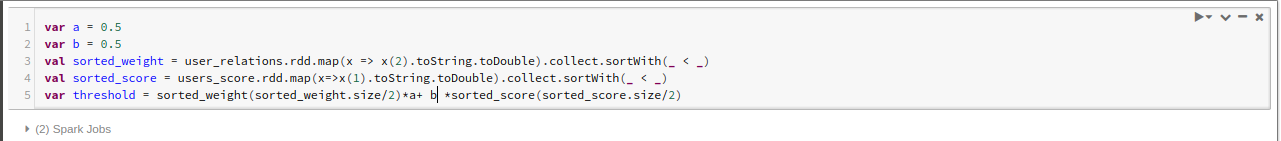
\includegraphics[width=1\linewidth,keepaspectratio]{command_24}
  \caption{Calcolo della soglia}
  \label{command_24}
\end{figure}
\clearpage

\subsection{Implementazione in Scala}
Per l'implementazione dell'algoritmo di \textit{spread}, in Scala, si è fatto uso
della funzione \textit{\textbf{Pregel}}, messa a disposizione dalle API di
\textit{\textbf{Graphx}}.\\
Pregel implementa uno scambio di messaggi tra nodi tramite l'utilizzo di tre
metodi:
\begin{itemize}
	\item \textbf{MergeMsg}: nel caso in cui il nodo riceve messaggi da più sorgenti
	definisce un criterio con cui selezionare solo un messaggio;
	\item \textbf{vProg}: definisce le azioni da compiere nel nodo alla ricezione del messaggio;
	\item \textbf{SendMsg}: definisce i valori da inserire nel nuovo messaggio ed
	il suo criterio di trasmissione.
\end{itemize}
L'esecuzione di \textit{\textbf{Pregel}} è suddivisa in \textbf{Super Step}.\\
In ogni super step, per ogni nodo che riceve un messaggio, sono eseguiti i metodi
sopra descritti.\\
Inoltre possono essere specificati altri parametri come: numero massimo di
iterazioni e messaggio iniziale.\\
Nella figura è riportato il codice per la definizione delle funzioni:
\textbf{MergeMsg}, \textbf{vProg} e \textbf{SendMsg}.
\begin{figure}[!htbp]
  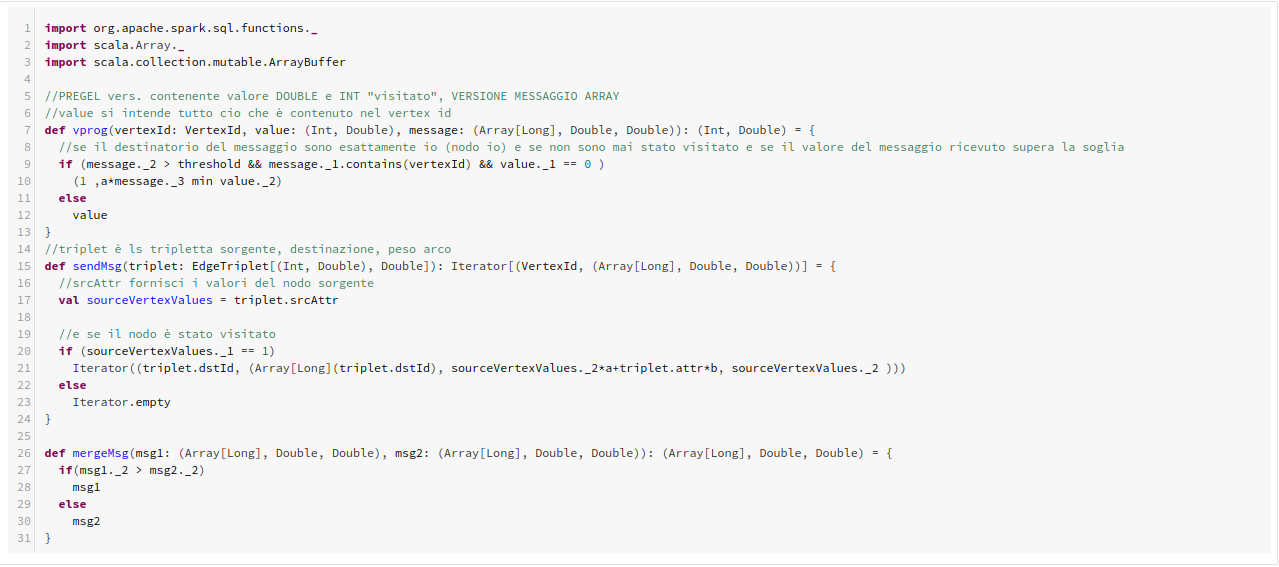
\includegraphics[width=1\linewidth,keepaspectratio]{command_25}
  \caption{Definizione MergeMsg, vProg, SendMsg}
  \label{command_25}
\end{figure}
\clearpage
Scendendo nel dettaglio, in \figurename~\ref{command_25} si osserva che:
\begin{itemize}
	\item in \textbf{MergeMsg} viene scelto, in caso di ricezione simultanea di
	messaggi, quello con valore maggiore;
	\item in \textbf{vProg} viene confrontato il secondo campo del messaggio ricevuto
	con la soglia, se il nodo è un nodo destinazione e se non è ancora
	stato influenzato, nel caso di esito di positivo, la variabile
	\textit{\textbf{influenced}} è settata ad 1 ed il valore del nodo è aggiornato
	con il \textit{min} tra il primo campo del messaggio(moltiplicato per 0.5) ed il suo score;
	\item in \textbf{SendMsg} ogni nodo che è stato influenzato invia un messaggio
	a tutti i suoi vicini.
\end{itemize}
Nel seguente codice è riportato l'algoritmo di \textit{Spread} per ogni
combinazione e l'estrazione del risultato finale avente maggiore copertura.
\begin{figure}[!htbp]
  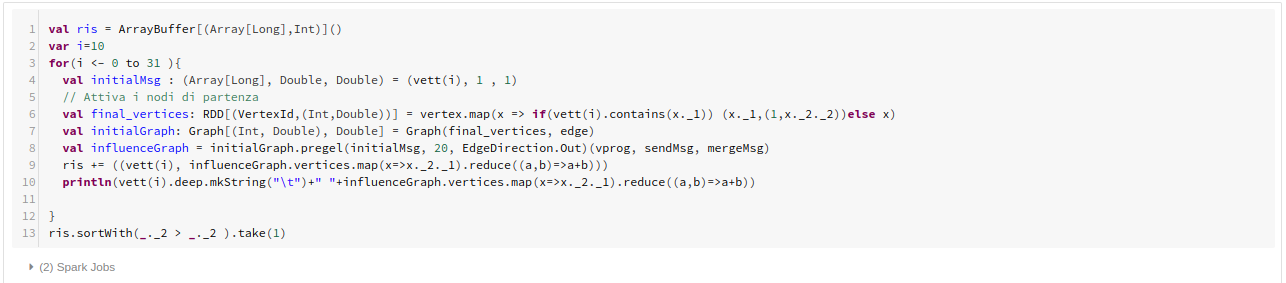
\includegraphics[width=1\linewidth,keepaspectratio]{command_26}
  \caption{Esecuzione Pregel}
  \label{command_26}
\end{figure}
\clearpage
